\documentclass[journal]{IEEEtran}
\usepackage{amsmath,amssymb,graphicx,booktabs,url,xcolor}
\usepackage[hidelinks]{hyperref}
\newcommand{\Pparams}{18,962}
\newcommand{\Dparams}{19,450}
\newcommand{\DevN}{319}
\newcommand{\NegN}{2689}
\newcommand{\SessionN}{13}
\newcommand{\MatchedN}{311}
\newcommand{\MatchedPoints}{2,756}
\newcommand{\AllPoints}{2,818}
\newcommand{\TrainN}{55,980}
\newcommand{\UsableTrainN}{55,915}
\newcommand{\CalN}{1,004}
\newcommand{\SelectionN}{1,031}
\newcommand{\HeldoutN}{1,985}
\newcommand{\Rmedian}{6.616}
\newcommand{\Pmedian}{5.905}
\newcommand{\Improve}{0.711}
\newcommand{\ImproveLow}{0.411}
\newcommand{\ImproveHigh}{1.174}
\newcommand{\RPCK}{63.733}
\newcommand{\PPCK}{67.341}
\newcommand{\PDdelta}{-0.525}
\newcommand{\PDlow}{-0.980}
\newcommand{\PDhigh}{-0.210}
\newcommand{\TranslationImprove}{7.439}
\newcommand{\Ptime}{13.661}
\newcommand{\Pfulltime}{15.352}
\newcommand{\Rtime}{9.733}
\newcommand{\Rfulltime}{11.217}
\newcommand{\PriorAbstract}{The P--prior median difference is 0.336 pixels (paired-session interval [0.063,0.585]). The interval favors the prior, not P. This is a fixed-budget development comparison.}
\newcommand{\PriorTrainingStatus}{All three matched-budget fits were completed; the learning curves are diagnostic, not a best-checkpoint selector.}
\newcommand{\ConfirmationAbstract}{Independent real-session confirmation is not yet available.}
\newcommand{\ConfirmationProtocol}{Independent confirmation is awaiting new data. The collection plan starts with 12 separate sessions and 15 prespecified frames per session, with at least 30 frames independently double annotated before blind adjudication. This is not a power guarantee. Predictions are hidden during annotation and the full panel must be frozen before evaluation. Existing FINAL-named manifests have unavailable membership and are not treated as independent observations.}
\newcommand{\ConclusionPrior}{The source-derived prior comparison quantifies a fixed-budget tradeoff, not converged-method superiority.}
\newcommand{\ConfirmationConclusion}{Independent real-session confirmation remains required.}
\newcommand{\RuntimePanelStatus}{The expanded panel was measured in the same session for all comparators.}

% Generated evidence status: not a manuscript acceptance/submission flag.
\newcommand{\DopeAbstractStatus}{For frozen DOPE on reused DEV, the conditional keypoint median is 12.585 pixels before refinement and 7.461 pixels for the mean of three P seed statistics; full-GT PCK10 is 19.872 and 36.775 percent, respectively. }
\newcommand{\DopeMainStatus}{For frozen DOPE on reused DEV, the conditional keypoint median is 12.585 pixels before refinement and 7.461 pixels for the mean of three P seed statistics; full-GT PCK10 is 19.872 and 36.775 percent, respectively. The tables retain missing predictions and unfavorable outcomes.}
\newcommand{\DopeConclusionStatus}{The DOPE measurements describe one additional fixed application; they do not establish arbitrary-backbone transfer, independent TEST generalization or stable physical T/R improvement.}

% Completed ResNet18 direct-estimator and frozen-refiner evidence, October 2026.
\newcommand{\ThirdEstimatorStatus}{The third application is a completed full-image, nine-landmark Simple-Baselines-derived ResNet18. Its frozen FULL estimator receives RGB and registered physical dimensions, and its primary transfer test adds the same image-feature local refiner without a second dimension input (P0). D0 is the matched direct-residual control. P5 and P5\_CONSTANT form a separate dimension-input extension. All real-image outcomes are reused-development evidence.}
\newcommand{\ResnetAbstractStatus}{For the third, dimension-conditioned ResNet18 estimator, the primary P0 refiner changes reused-DEV conditional median error from 8.001 to 7.143 pixels and full-denominator PCK10 from 54.68\% to 58.28\%; reconstructed-reference translation and canonical camera-facing-frame C2 rotation medians change from 11.007~cm/3.252~deg to 10.001~cm/3.018~deg.}
\newcommand{\ResnetMainStatus}{The ResNet18 FULL estimator and all twelve D0/P0/P5/P5\_CONSTANT head fits completed. P0 is the primary third-backbone transfer arm; it improves central 2D development error and PCK10, while its translation interval includes zero. P5 is reported only as a separate dimension-conditioned-head extension because P5--P5\_CONSTANT does not establish stable joint 2D/T/R improvement.}
\newcommand{\ResnetConclusionStatus}{A third frozen feature interface supports the primary P0 refinement result on reused DEV, but the separate P5--P5\_CONSTANT comparison does not establish a robust incremental benefit from dimensions or stable physical T/R improvement.}
\newcommand{\ResnetBaselineStatus}{The completed direct-estimator study trains CONSTANT, SHAPE and FULL arms for a fixed 10 epochs on 55,980 synthetic TRAIN images (34,990 updates and 559,800 exposures per arm). All share seed 42, ImageNet ResNet18 initialization, identical source order and photometric augmentation. FULL supplies normalized $\log W$, $\log D$, $\log H$, $\log(W/D)$ and $\log(H/\sqrt{WD})$ to a decoder FiLM block; SHAPE keeps only the two ratios and CONSTANT supplies zeros. Epoch 10 is fixed using no real-image selection.}

\title{Feature-Reusing Local Keypoint Refinement for Monocular Pallet Pose Estimation: Frozen Estimator Applications}
\author{Internal research draft---author details pending\thanks{Not submitted. Independent confirmation and author declarations remain subject to the evidence status reported in this draft.}}
\markboth{Internal Revision for Author Review, October 2026}{Fixed Local Pallet Refinement}
\begin{document}
\maketitle
\begin{abstract}
Accurate image landmarks are important to monocular pallet pose measurement, but improving localization need not require changing an established detector. We study a fixed, synthetic-supervised local keypoint refiner that reuses two feature scales of a frozen RGB estimator. In the completed YOLO application, the \Pparams{}-parameter module predicts a distribution over local corner displacements while preserving bounding boxes, confidence scores, instance selection, and the center landmark. For this application, on \DevN{} reused development images from \SessionN{} sessions, the mean over three independently trained seeds of pooled landmark median error changes from \Rmedian{} to \Pmedian{} pixels. The paired-session interval for the reduction is [\ImproveLow{},\ImproveHigh{}] pixels. Complete-denominator keypoint accuracy, error tails, geometry-reference pose errors, and desktop latency are reported separately. A matched-evidence direct regression control and a source-derived PoseFix pallet adaptation test distinct refinement alternatives. \PriorAbstract{} These measurements establish the scope of the development evidence, not an unseen-session guarantee. \ConfirmationAbstract{} The extension applies the same correction principle to a separately frozen DOPE estimator with new source-trained heads and explicit missing-point accounting. \DopeAbstractStatus{} \ResnetAbstractStatus{} Neither a universal model-agnostic result, an original expectation operator, nor operational handling reliability is claimed.
\end{abstract}
\begin{IEEEkeywords}
Monocular vision, pallet pose, keypoint refinement, synthetic supervision, feature reuse, measurement evaluation.
\end{IEEEkeywords}

\section{Introduction}
Pallet localization provides geometric input to inspection, tracking, and material-handling systems. A monocular RGB camera offers a compact sensing interface, but image-level detection is not the same quantity as accurate geometric measurement. The same correctly detected instance can have displaced corners; a downstream perspective-n-point (PnP) solver can amplify some image errors depending on geometry and viewing configuration. It is therefore useful to distinguish detection, conditional landmark precision, and pose measurement when evaluating a refinement method.

Synthetic training can supply image supervision without manually annotating every pallet training image. Synthetic RGB pallet pose estimation is already established, for example through the Euro-pallet study of Knitt et al.\ \cite{knitt}. We do not claim its invention, a measured reduction in annotation labor, or a universal synthetic-to-real solution. Instead, we ask a narrower question: can a small local module improve the residual geometry of a fixed estimator while leaving its detection outputs unchanged?

We investigate the already-trained point refiner P. It reads existing detector features and scores candidate displacements around each predicted corner. The detector is frozen, but this is not a guarantee that corrected geometry is harmless: a wrong displacement can still degrade a keypoint or a pose. Our evaluation therefore retains tails, individual sessions, and complete ground-truth denominators alongside the central error statistic. The original application depends on the YOLO feature interface. A second, separately specified DOPE application tests whether the same local readout principle remains useful with different frozen features and error patterns. It requires a new adapter and new heads, not zero-shot transfer of the YOLO weights. A finite set of fixed applications cannot establish universal model-agnostic behavior.

\ThirdEstimatorStatus{}

The contributions are an explicitly specified feature-reusing refinement interface, within-estimator comparisons of the local distribution readout with a direct residual control, and an auditable protocol tying original-pixel outputs to failure-aware geometry and measured cost. Historical YOLO line-structured and prior-derived comparisons remain visible. The second-estimator claim is conditional on the separately reported DOPE results, including adverse outcomes. These are system and empirical contributions to be assessed against the evidence. We do not introduce a new expectation operator, a low-rank adaptation algorithm, or a new safety controller. Figure~\ref{fig:pipeline} separates the learned correction from the frozen detector and the geometry inputs.

\begin{figure}[t]
\centering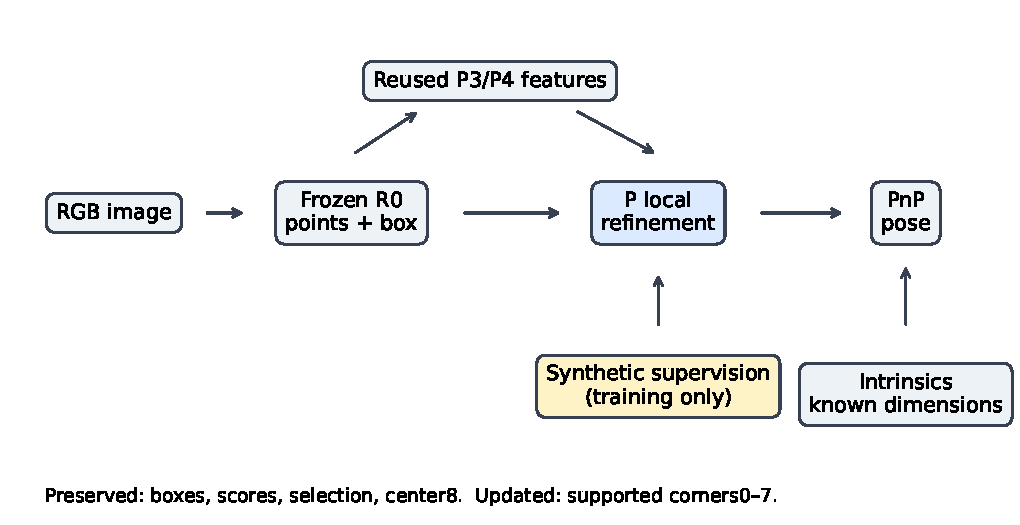
\includegraphics[width=\columnwidth]{figures/pipeline.pdf}
\caption{Information paths of the completed YOLO application; the DOPE extension has its separate frozen adapter. P uses image features and predicted points/box. Camera intrinsics and registered physical dimensions enter the downstream pose solver, not P. Synthetic labels supervise P during training only. Boxes, scores, selected instance, and center are preserved; corner geometry can change.}
\label{fig:pipeline}
\end{figure}

\section{Related Work and Comparison Scope}
\subsection{Pallet perception and synthetic supervision}
DOPE\cite{dope} estimates semantic cuboid landmarks from RGB. Knitt et al.\ \cite{knitt} trained a DOPE-based pallet estimator using synthetic imagery and evaluated RGB Euro-pallet pose. More recently, Miura et al.\ \cite{miura} studied monocular pallet pose using metric-depth predictions and ground-plane information. These works motivate the application and establish that RGB pallet estimation and synthetic data are not new in themselves. Their datasets and auxiliary information differ from ours; published numbers are not subtracted from the present development results.

\subsection{Pose and coordinate refinement}
PoseFix\cite{posefix} refines an input pose using the image and a separate backbone. Its human-pose training procedure synthesizes pose errors from human-keypoint statistics. Our purpose adaptation replaces those human assumptions with frozen source-training predictions from the pallet detector. It is named \emph{PoseFix-derived pallet9, matched-exposure adaptation}, not a reproduction of the original human benchmark. Integral regression\cite{integral} establishes differentiable coordinate expectation as prior art. P applies an expectation to candidate displacements; the expectation itself is not a claimed invention.

CRT-6D\cite{crt} uses object-surface keypoint features in cascaded pose refinement. It is relevant to sparse feature-based correction, but has a different object-surface and pose contract. The inspected official repository at the recorded commit contains no executable network; no substitute transformer is reported as CRT-6D. Our named prior experiment is limited to the declared PoseFix-derived family rather than expanding a benchmark after seeing results.

\subsection{Feature reuse and small side networks}
Side-tuning\cite{side} relates to adapting a fixed representation through a separate learned path. P shares the general motivation of retaining a backbone and training a smaller addition. Nevertheless, P does not implement LoRA, and no new parameter-efficient fine-tuning benchmark is established. Both P and the direct control D have small learned heads. Their difference therefore cannot be attributed simply to parameter efficiency. Freezing the backbone also does not make inference overhead zero.

\section{Fixed Refinement Method}
\subsection{Sensor, detector, and coordinates}
The historical baseline R0 is a YOLO26n pose estimator producing a box, confidence, and nine points per candidate instance. The selected instance is the highest-confidence prediction under the existing pipeline. Corner indices 0--7 retain the registered cuboid convention, and index 8 retains the established center definition. The wrapper does not use a ground-truth box or pose to select the input instance. Ground truth is used downstream for training supervision and evaluation matching only.

R0 was initialized from a pretrained YOLO26n pose checkpoint, and its stored provenance identifies COCO-pose training in that checkpoint. The pallet run also records pretrained initialization. Thus, ``synthetic-supervised refinement'' refers to the training of the additional module, not a claim that no real annotations ever contributed to the full estimator. Real labels are also used in development and evaluation. R0 is not retrained in the present comparison.

The historical image pipeline is preserved: rectangular detector preprocessing at the registered input size, stride-aware padding, and original-image restoration. Prepared synthetic images already include their recorded reflection padding and are not padded a second time. Let $A$ be the diagonal image-to-network scaling matrix and $\mathbf{o}$ its offset. Original points $\mathbf{p}$ and network-input points $\tilde{\mathbf{p}}$ satisfy $\tilde{\mathbf{p}}=A\mathbf{p}+\mathbf{o}$. YOLO letterboxing gives $A=gI$; the DOPE raster can have unequal actual horizontal and vertical scales. Corrections use $A^{-1}$ on displacements and add them to the retained original points. A zero correction therefore preserves the exact baseline coordinates.

\subsection{Local candidate evidence}
P adapts P3/P4 features with small learned channel projections. Around each valid corner, 13 directions and 17 radii define 221 displacement candidates within 0.08 predicted-box diagonal. A zero-displacement null candidate completes the 222-way distribution. Each non-null candidate reads a $4\times8$ stencil from both feature scales using the registered bilinear sampling geometry. A shared patch encoder and corner-role/context features feed candidate and null scorers. No explicit edge or Hough representation is required by P.

Let $d_b$ denote the predicted box diagonal in network-input pixels, $\mathbf{v}_j$ the normalized candidate offsets, and $z_{kj}$ the score for corner $k$. For the frozen temperature $T$ and scale $\lambda$, the proposed displacement is
\begin{equation}
\boldsymbol{\delta}_k=\lambda d_b\sum_j\frac{\exp(z_{kj}/T)}{\sum_l\exp(z_{kl}/T)}\mathbf{v}_j.
\end{equation}
The null candidate has $\mathbf{v}_{\mathrm{null}}=\mathbf{0}$. Given an original-image diagonal $d_I$ and frozen cap fraction $\alpha$, movement and restoration are
\begin{align}
\boldsymbol{\Delta}_k&=A^{-1}\boldsymbol{\delta}_k,\\
\bar{\boldsymbol{\Delta}}_k&=\boldsymbol{\Delta}_k\min\left(1,\frac{\alpha d_I}{\|\boldsymbol{\Delta}_k\|_2}\right),\\
\mathbf{p}'_k&=\mathbf{p}_k+\bar{\boldsymbol{\Delta}}_k,
\end{align}
with unit scaling for a zero movement and no clipping when the selected cap is absent. Historical YOLO P retains its selected $\lambda=1$, $\alpha=0.01$, and per-seed temperatures. DOPE uses the same source-only selection grid; its selected values are supplied with its own result records. Unsupported points are unchanged; point 8 is copied exactly. Detection boxes, confidences, candidate order, and nonselected points are preserved. These contracts do not imply unchanged or always improved 6D geometry.

\subsection{Training and internal controls}
\begin{figure}[t]\centering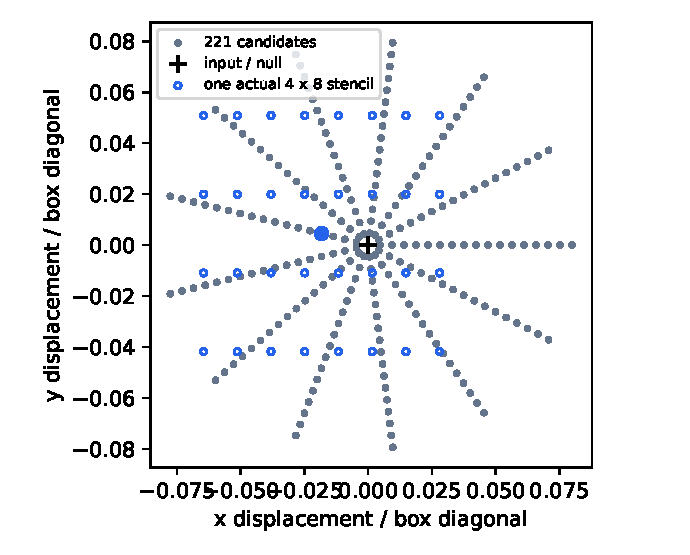
\includegraphics[width=\columnwidth]{figures/candidate_sampling.pdf}
\caption{The implemented candidate lattice and one actual sampling stencil in box-diagonal units. The blue stencil is shown at a fixed candidate index, not selected for performance. The probability expectation in (1) combines candidate displacements; no illustrative weights are presented as measured outputs. Geometry and source hashes are recorded in FIGURE\_MANIFEST.json.}\end{figure}
P learns a soft distribution over candidate displacements from synthetic corner residuals. The finite target support and per-frame reduction are retained from the fixed implementation. The historical YOLO P, D, and L fits each use their recorded three seeds and fixed exposure budget; those models are not retrained. YOLO P has \Pparams{} learned parameters. D reuses the same sampling and shared feature descriptors, but regresses normalized corner residuals with an L1 objective. The YOLO D instance has \Dparams{} parameters and an unbounded raw output, in contrast to P's candidate convex hull. This is a comparison of readout/supervision packages, not a causal ablation of softmax alone.

L is the historical line-structured internal control. Its results are retained to show that explicit line structure has not established an all-metric benefit in this configuration. Earlier Hough, active-adaptation, and replay investigations are part of the research history, not new primary comparisons in this manuscript. No unfavorable historical outcome was deleted.

For a supported corner with target residual $\mathbf{r}_k$, P's target mass is
\begin{equation}
q_{kj}=\frac{\exp[-\|d_b\mathbf{v}_j-\mathbf{r}_k\|^2/(2\sigma^2)]}{\sum_l\exp[-\|d_b\mathbf{v}_l-\mathbf{r}_k\|^2/(2\sigma^2)]},\quad \sigma=0.08d_b/17.
\end{equation}
Cross-entropy is averaged over supported corners within each frame and then over frames with support. This smooth finite-candidate target differs from D's direct residual L1 supervision. Its existing settings are retained, not newly optimized here.

\subsection{Second fixed estimator: DOPE adapter}
The second application freezes an existing six-stage pallet DOPE checkpoint and changes the feature adapter rather than the correction principle. The checkpoint is identified by SHA-256 in the protocol; no DOPE weight is updated by the refiner fits. We use the existing semantic-channel local-peak decoder at threshold 0.3. This implementation does not run affinity-based multi-object grouping. Its fixed box is the hull of at least three valid predicted corners, and its score is the maximum corner belief. Thus, this is an application to the declared single-pallet DOPE pipeline, not a reproduction of every original DOPE inference option or a detector-ranking experiment.

The two frozen VGG taps are post-ReLU layers 17 and 26, with 256 channels at stride 4 and 128 at stride 8. Learned projections map both to the same 16-channel evidence interface used by P and D; the shared encoded width is 24. The candidate lattice, stencil geometry, corner ordering, null candidate, losses, and displacement restoration remain as specified above. Input-channel counts change the number of learned parameters; the YOLO count is not assigned to the DOPE heads. A matched-evidence D control is trained for each DOPE seed. L and the separate PoseFix-derived comparator are historical YOLO controls and are not silently presented as new DOPE experiments.

The fixed adapter applies reflection padding of 100 pixels to native real RGB, resizes the padded canvas back to the native size, then uses the recorded shortest-side-400, multiple-of-eight raster. Synthetic source RGB already contains this reflection preparation and receives no second padding. The exact composed affine, including actual raster widths and heights, maps predictions back to the caller's coordinates. Training retains the source preparation; DEV restores unpadded original pixels before measurement. The inference preprocessing and normalization are checked against the selected existing inference path, not claimed to be byte-identical to the original augmented DOPE training pipeline.

Predicted missing points stay missing. P and D cannot create a previously absent corner, change the fixed hull or score, or replace the center landmark. A point without the required feature support is copied rather than supplied with a target-derived value. These invariants isolate local refinement but also bound what it can repair: low coverage cannot be hidden by reporting only an accurate surviving subset. Camera intrinsics and physical dimensions remain exclusive to downstream PnP.

\subsection{Third application: full-image ResNet18}
The third estimator is a full-image pallet adaptation of Simple Baselines\cite{simplebaseline}, using an ImageNet-initialized ResNet18 body, three 256-channel stride-two deconvolutions, and nine stride-four heatmaps. It uses no YOLO detection or ground-truth crop. Prepared RGB is aspect-fitted to $384\times512$ with centered letterboxing and ImageNet FP32 normalization. Targets are continuous Gaussians with output-grid sigma 2; the masked half-MSE retains all nine channel slots and every frame in its denominator. Decoding uses the fixed argmax/interior quarter-pixel rule and peak threshold 0.1, with explicit missingness and exact affine restoration.

\ResnetBaselineStatus{} After the baseline is frozen, P/D read layer2/layer3 features (128/stride8 and 256/stride16) under the same fixed three-seed head budget. Each application uses independently initialized heads; no YOLO or DOPE head is a warm start.

\subsection{Purpose-adapted prior comparator}
The historical YOLO prior uses the official PoseFix ResNet152 arrangement, an aspect-corrected and 1.25-expanded predicted-box RGB crop of $384\times288$, and nine Gaussian input pose maps. It adds ImageNet TF-Slim initialization, masks center loss and restores the original center. Human swap/inversion noise is replaced by actual frozen source-detector errors. Operator and training parity checks for the source-based PyTorch port, including the effective fused-BN epsilon and target-boundary handling, are detailed in the supplement.

Its declared budget is three seeds of 6,000 Adam updates at batch 16 in the exact historical P sample order, using the final checkpoint. This is a matched-exposure adaptation rather than the original 140-epoch human-pose protocol or a claim of convergence. \PriorTrainingStatus{}

\subsection{Downstream geometric measurement}
The unchanged prediction-only selector uses the registered camera intrinsics and physical pallet dimensions to select its dimension hypothesis. The selected cuboid is solved using the canonical SQPnP/RefineLM path. Intrinsics and dimensions are not neural inputs to P or D. Ground truth does not choose the prediction's most favorable pose hypothesis. Current reference poses are reconstructed from manual image points and known geometry, rather than obtained from an independent physical 6D instrument. Near-square axis confusion is not newly excused by adding a symmetry minimization.

\section{Datasets and Measurement Protocol}
\subsection{Source exposure and rule selection}
\begin{table}[t]\centering\caption{Historical YOLO comparator contract. All added heads use zero real-pallet training examples; R0 upstream COCO-pose initialization is shared within this panel. Geometry enters PnP, not the heads. DOPE uses its own frozen checkpoint.}\label{tab:inputs}
\small\begin{tabular}{lll}\toprule Method & Added inference input & Added pretraining\\\midrule
R0 & none & none\\
P/D/L & R0 P3/P4, pose/box & none\\
Prior & RGB crop, pose/box & ImageNet classes\\\bottomrule\end{tabular}\end{table}
For historical YOLO, the source manifest contains \TrainN{} training records, with \UsableTrainN{} usable matched training rows, and calibration/selection/heldout partitions of \CalN{}/\SelectionN{}/\HeldoutN{} records. Source images, labels, row order, and completed model choices are hash-bound. Actual RGB crops, rather than guessed images reconstructed from cached features, are used for the prior backbone. Synthetic source subsets are historically reused and are not described as universally untouched data.

The prior shares the existing synthetic-only lambda/cap grid, objective, and tie rule. Coordinate outputs do not receive a fabricated temperature sweep. Raw prior and capped-wrapper results are reported separately. Heldout results are computed after selection; DEV does not choose the checkpoint, learning rate, noise model, or wrapper. The historical model panel is frozen before any independent confirmation annotations may be opened; the DOPE extension also freezes source-selected rules before its DEV replay.

\subsection{Fixed DOPE source budget and selection}
DOPE uses the same 60,000-record synthetic RGB source manifest: 55,980 training, 1,004 calibration, 1,031 selection, and 1,985 heldout records. A usable training row needs the frozen predicted hull to meet IoU 0.5 with the source object and at least one jointly valid corner. Its usable count is estimator-specific and must not inherit the historical YOLO count. Each of three seeds trains a fresh P and a fresh D for exactly 6,000 AdamW updates of nominal batch 16. Within a seed they share the exact row sequence and frozen feature evidence, giving 96,000 nominal source exposures per head. Cross-estimator usable rows need not coincide. Frozen VGG prefixes run online; the DOPE stage heads are not rerun inside these training steps. Feature maps use the original FP16 roundtrip, with FP32 heads and no mixed-precision head training.

The learning-rate, warmup, decay, gradient clipping, and final-checkpoint rule are fixed in advance; no DEV-based early stopping or architectural sweep is allowed. A discarded two-update smoke check is a separate implementation check, not a seventh reported fit or a warm start. P temperature is selected on the calibration partition from $\{0.5,1,2,4\}$ using supported-frame target cross-entropy. D has no temperature selection. Each family selects one three-seed mean rule on the selection partition from $\lambda\in\{0,0.0625,0.25,1,4\}$ and cap fractions $\{\mathrm{none},0.01\}$. The fixed tie rule favors smaller $\lambda$ and then the stricter cap. Missing source supervision contributes the declared failure penalty; no real image chooses a wrapper. Heldout measurements follow rule freezing and remain historically reused source data.

The baseline-training budgets are not matched: the DOPE checkpoint ending in epoch 0060 was produced by the inclusive 0--60 loop, whereas YOLO uses its selected \texttt{best.pt}. Shared source imagery and matched P/D head exposure do not establish equal baseline optimization, augmentation, pretraining, or compute. The supplement records this distinction alongside the source and checkpoint hashes.

\subsection{Development population and supervision}
The historical YOLO positive development panel has \DevN{} images in \SessionN{} recorded sessions; \NegN{} negative images accompany the detection-preservation audit. In that historical panel there are \MatchedN{} matched positive frames and \MatchedPoints{} supervised points for conditional precision, versus \AllPoints{} supervised points in the complete ground-truth denominator. Point supervision is the original label contract and is not renamed as measured physical visibility. Visible boundaries, inferred amodal corners, and unavailable landmarks require distinct interpretation in new annotation QA.

The DOPE extension reuses the identical 319 positive images and 2,818 supervised points, but reports its own matched and missing counts. Canonical conditional precision requires the fixed box match and all nine predicted points finite; a separate partial-point diagnostic cannot replace it. P and D preserve this baseline support within DOPE, without requiring equal support across estimators. There is no new DOPE negative-image/AP experiment.

The primary statistic pools supervised original-pixel Euclidean errors within each model seed, computes its median, and then averages the three seed statistics. It is neither an ensemble prediction nor the average of frame medians. Its conditional precision denominator excludes unmatched frames, which is why complete-denominator PCK is also required. For threshold $t$,
\begin{equation}
\mathrm{PCK}_{t}=\frac{\sum_{i,k}h_{ik}(t)}{N_{\mathrm{GT}}},
\end{equation}
where missing predictions, unmatched top instances, and nonfinite points contribute zero hits, not zero error. Matching remains at the registered box IoU threshold. If any support differs, an intersection-only median cannot replace this failure-aware report. In the DOPE extension a conditional paired interval is not computed when its per-frame support differs; the mismatch is reported alongside full-denominator PCK and pose coverage.

Registered object sizes and the per-annotation camera intrinsics are tabulated in the supplement. They are inputs to this geometry-reference evaluation, not newly certified metrology. The canonical solver uses no distortion coefficients; independent camera calibration uncertainty is not established by these annotation records. The declared long-axis benchmark admits a half turn but not a quarter turn. In particular, the wood object's visual symmetry under a half turn is unverified. Such conventions do not establish physical fork-entry interchangeability.

\subsection{Uncertainty and pose metrics}
We use 10,000 paired session bootstrap draws with seed 20260914, applying each draw's frame/session multiplicities to every model seed. The P--R0 statistic compares against one baseline, not three copies treated as independent models. P--D and P--prior are secondary development contrasts. Secondary intervals are not multiplicity-adjusted and are not confirmatory superiority, equivalence, or noninferiority tests. The reused development data cannot be made independent by specifying this protocol after previous analyses.

Rotation, yaw, translation, 3D IoU, and symmetry-aware ADD AUC are evaluated under the existing geometry-reference convention. Pose coverage and 2D matching are different denominators: a solver can return a pose from an incorrectly matched top detection. Translation-error changes in centimeters can be expressed in millimeters, but a pixel reduction cannot be converted to one universal millimeter gain. No insertion trials or independently instrumented physical pose measurements are included.

\subsection{Cost and independent confirmation}
\RuntimePanelStatus{}

Desktop latency starts from decoded BGR input and includes preprocessing, R0, refinement, and restoration. Canonical PnP time is recorded separately and added for the whole estimation path. Loading and image decoding are excluded. The protocol uses the historical 26 images, 20 warmups per model, five balanced cyclic/reversed blocks, batch one, and four Torch intra-operation CPU threads. OpenCV/inter-operation observations were saved only for the subsequent isolated-memory phase, not the timing phase; four is not a universal process thread limit. Training and scoring do not overlap timing. Display/remote desktop activity is disclosed; no fastest repeat is selected. Prior-specific cropping and its separate backbone are included, while P recomputes detector features instead of reading a training cache. The supplement records numerical replay checks and the recovery of memory measurement after the completed timing panel.

The DOPE timing protocol separately measures the fixed seed-1 DOPE, DOPE+D, and DOPE+P paths on the first two manifest-ordered images per session (26 images), after 20 warmups and in five balanced cycles. Its actual times, device observations, coverage, and replay checks must be reported before any cross-estimator cost claim. Historical YOLO timing is not reused as DOPE timing.

\ConfirmationProtocol{}

\section{Results}
\IfFileExists{figures/accuracy_latency.pdf}{\begin{figure}[t]\centering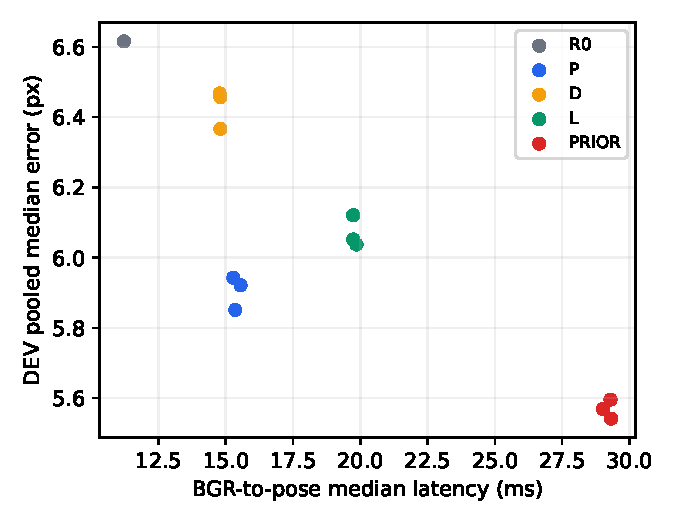
\includegraphics[width=\columnwidth]{figures/accuracy_latency.pdf}\caption{Historical YOLO per-seed DEV median against same-session median full-path latency. Lower is preferable on both axes. Each seed is a point, not a timing-selected winner or ensemble; separate-backbone prior cost is included. Source result/runtime hashes are recorded in FIGURE\_MANIFEST.json.}\end{figure}}{}
\subsection{Completed historical YOLO comparisons}
Table~\ref{tab:accuracy} summarizes the original-pixel and geometry-reference measurements. Complete per-seed tables, extra PCK thresholds, coverage, and uncertainty are supplied in the supplement. P changes the baseline pooled median from \Rmedian{} to \Pmedian{} pixels, a reduction of \Improve{} pixels. Its paired-session reduction interval is [\ImproveLow{},\ImproveHigh{}] pixels. PCK10 changes from \RPCK{}\% to \PPCK{}\%. These figures describe the present development panel only.

\begin{table}[t]\centering\caption{Reused DEV: seed-mean statistics, not an ensemble. Translation is against the geometry reference. NM means not measured in this build.}\label{tab:accuracy}
\small\begin{tabular}{lrrrr}\toprule
Model & Median & P90 & PCK10 & Trans.\\
 & px & px & \% & cm\\\midrule
R0 & 6.616 & 38.670 & 63.73 & 7.897 \\
P mean & 5.905 & 37.766 & 67.34 & 7.153 \\
D mean & 6.430 & 37.566 & 64.57 & 7.597 \\
L mean & 6.070 & 37.320 & 66.78 & 7.548 \\
PRIOR mean & 5.569 & 37.227 & 68.41 & 6.895 \\
\bottomrule\end{tabular}\end{table}


The P--D median difference is \PDdelta{} pixels, with paired-session interval [\PDlow{},\PDhigh{}]. This supports a lower central development residual for P than this fixed direct control. It does not prove that direct regression as a method class is inferior. D has a slightly lower observed P90, and the P--D tail interval includes zero. D also has lower measured desktop latency. There is therefore no all-metric dominance claim. The internal line control also has a lower observed P90 than P.

Figure~\ref{fig:sessions} retains every recorded session. The \texttt{eval\_noapril} session has an adverse P--R0 central effect; the other twelve observed sessions improve. Leave-one-session-out estimates remain favorable in this panel, but such deletion diagnostics are not new independent datasets. No unfavorable session is removed from the aggregate.
\begin{figure}[t]\centering
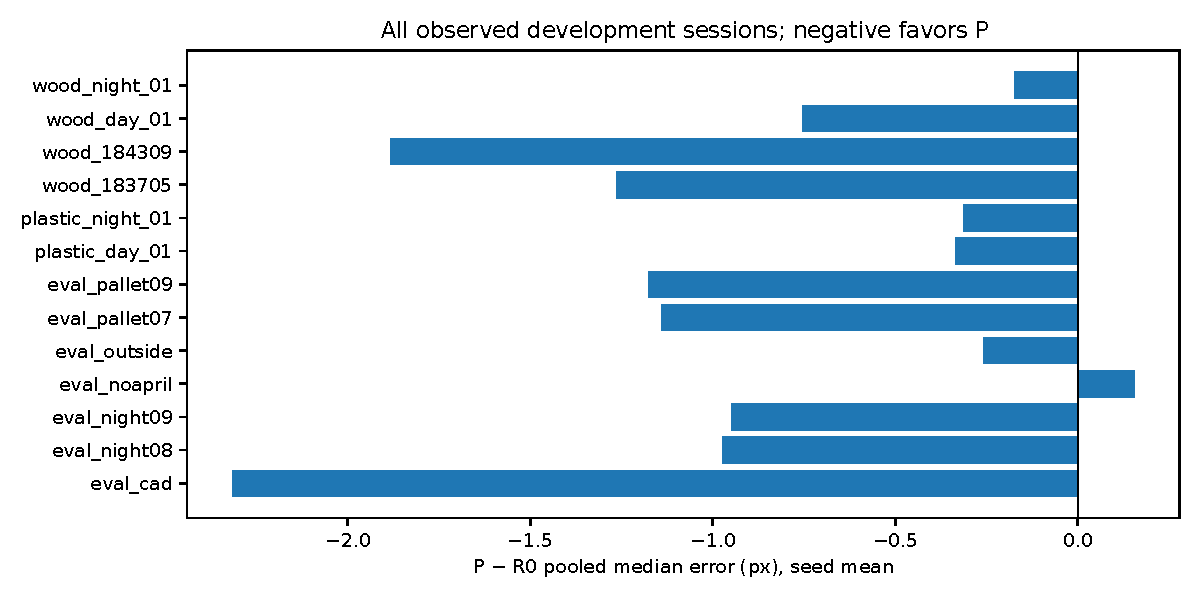
\includegraphics[width=\columnwidth]{figures/session_effects.pdf}
\caption{P--R0 development median effects by recorded session. Negative values favor P. These are descriptive effects from the reused panel, not independent confirmation intervals. All sessions are retained.}
\label{fig:sessions}\end{figure}

The seed-mean reduction in geometry-reference translation median is \TranslationImprove{} mm. This is a change in error statistics against a reconstructed reference, not measured insertion improvement. It cannot establish physical metrology accuracy independently of the image-label and reference-construction uncertainty.

\subsection{Prior-derived comparison}
The prior checkpoints were fixed at the final training update; only the wrapper rule was selected on synthetic data. The selected wrapper has lambda 1.000 and cap fraction 0.01. Raw and wrapped outputs are separate supplementary rows. All wrapped prior seeds retain the baseline matched supervision support, with no nonfinite supervised coordinates. The P--prior paired median difference is 0.336 px, with session interval [0.063, 0.585] px. This interval favors the prior, so P is not the most accurate comparator under this central-error criterion. A negative contrast favors P; a positive contrast favors the prior. The complete-denominator PCK, tail and pose rows must be considered alongside the median. Six thousand updates per seed do not certify saturation or reproduce the original 140-epoch protocol.


\subsection{Second-estimator development evidence}
\DopeMainStatus{}
\noindent DOPE measurement status: pending. The reserved result table will contain baseline DOPE and three-seed D/P statistics, with matched counts, all-GT PCK and pose coverage. No zero or historical YOLO value represents an unmeasured DOPE result.

The supplement reports the full per-seed table, paired intervals, source-heldout statistics and selected wrappers.
Within DOPE, central residuals, complete-denominator accuracy, tails, and pose coverage are separate outcomes. A lower conditional median alone cannot establish a net sensing improvement when missing predictions remain. Across estimators, unequal baseline errors, boxes, features, and upstream training prevent a causal attribution to backbone identity. Any favorable DOPE effect supports this fixed application only; a null or adverse result remains part of the same experiment.

\subsection{Third-estimator development evidence}
\ResnetMainStatus{}
\begin{table*}[t]\centering\small
\caption{Primary ResNet18 frozen-estimator transfer on reused DEV319. FULL is the dimension-conditioned direct estimator; D0 and P0 are means of three per-seed statistics, not prediction ensembles. P0 is the primary local-refinement arm and has no additional dimension input. Conditional 2D errors require the fixed baseline hull match; PCK10 retains all 2,818 supervised landmarks. Pose errors use the reconstructed geometry reference, R is canonical MAIN camera-facing-frame C2 rotation, and all arms have 319/319 solver coverage.}\label{tab:resnet}
\begin{tabular}{lrrrrrrr}\toprule
Arm & Med. px & P90 px & PCK10 \% & Match/319 & T cm & R-C2 deg & C2-aware ADD AUC\\\midrule
FULL baseline & 8.001 & 52.054 & 54.68 & 299 & 11.007 & 3.252 & 0.31296\\
D0 mean & 7.852 & 51.928 & 55.26 & 299 & 9.837 & 3.218 & 0.32604\\
P0 mean & 7.143 & 52.086 & 58.28 & 299 & 10.001 & 3.018 & 0.34219\\
\bottomrule\end{tabular}
\end{table*}

The supplement retains all seven arms, paired intervals, source evidence, the complete baseline learning curve and actual timing. Cross-estimator comparisons remain descriptive because their baseline training and matched supports differ.

\subsection{Efficiency and accuracy--cost tradeoffs}
\RuntimePanelStatus{}

\begin{table*}[t]\centering\small
\caption{Integrated same-image desktop latency (ms), representative seed 1 for learned heads. All methods use the same 26 decoded BGR images, batch one, 20 warmups and five retained repeats. Loading and decoding are excluded; model-specific preprocessing, 2D output and canonical prediction-only PnP are included.}\label{tab:runtime}
\begin{tabular}{lrrrr}\toprule
Method & 2D med. & 2D P90 & Full med. & Full P90\\\midrule
YOLO R0 & 9.554 & 11.594 & 11.092 & 13.184\\
YOLO+P1 & 13.174 & 15.468 & 14.779 & 16.959\\
DOPE & 62.894 & 76.766 & 64.585 & 78.870\\
DOPE+P1 & 66.291 & 80.003 & 67.411 & 81.361\\
ResNet18 FULL & 7.835 & 10.432 & 9.453 & 12.146\\
ResNet18+P0-S1 & 10.520 & 13.565 & 12.193 & 14.982\\
\bottomrule\end{tabular}
\end{table*}

P's selected seed1 is the prespecified deployment representative; it must not be confused with the seed mean. Its desktop BGR-to-2D and PnP-inclusive median times are \Ptime{} and \Pfulltime{} ms, compared with \Rtime{} and \Rfulltime{} ms for R0 in the cited timing session. Allocator memory is reported separately from whole-device memory, which also includes the display and other software. The tables do not extrapolate to Jetson, report unmeasured energy savings, or infer operational throughput from an isolated cached tensor.

The separate DOPE and ResNet18 seed-1 timing panels, including all pose failures, full-path timings and coordinate replay checks, are reported in the supplement. Their baselines and feature extraction paths differ; historical YOLO timing is not a substitute for either measurement.

\subsection{Independent confirmation}
Not yet measured: no independently reviewed capture/annotation panel is available. The proposed collection count is a plan, not a completed experiment. Development observations are not relabeled as confirmation results.


\section{Limitations and Interpretation}
First, the primary development improvement is conditional on matched supervision and on a historically selected model family. Complete-denominator PCK limits one failure mode of optimistic reporting, but does not turn reused DEV into a confirmation set. The session intervals condition on only thirteen observed sessions and three trained seeds; they do not quantify every deployment shift.

Second, the comparison contracts differ in useful ways that must remain visible. P reads internal R0 features; the PoseFix-derived prior computes a separate RGB representation and adds ImageNet pretraining. D has a different output support and loss. Equal source exposure is not equal compute or equal optimization difficulty. None of these comparisons identifies a universal architectural optimum. Bounded prior learning curves diagnose progress but cannot certify full convergence.

Third, current pose errors are measured against a geometry-reconstructed reference. Annotation ambiguity, calibration, object dimensions, and reference construction can affect interpretation. Independently blinded duplicate labels and reviewed capture lineage are required for new confirmation; physical 6D accuracy would require additional metrology. Neither preserved detections nor improved median error guarantees harmless tails, correct pallet axes, or safe handling.

Finally, each application is tied to a declared frozen feature interface and a desktop environment. The DOPE application requires its own channel/stride adapter, missing-point policy, new head fits, and decoder audit; it is not plug-and-play evidence for an arbitrary estimator. Reusing DEV for the second application does not create independent confirmation. Embedded export parity and Jetson latency are not measured. The work provides an auditable sensing experiment, not a demonstrated control system. The author team must assess whether the remaining independent evidence and scientific contribution are sufficient for submission; compilation and formatting checks are not an acceptance decision.

\section{Conclusion}
The completed YOLO application of a fixed feature-reusing point refiner improves the central landmark residual on the reused pallet development panel with a measured desktop cost. The preserved detection interface, failure-aware denominators, internal controls, and source-derived prior comparison make the scope of this claim explicit. \ConclusionPrior{} \ConfirmationConclusion{} \DopeConclusionStatus{} \ResnetConclusionStatus{} Further claims about independent generalization, physical sensing accuracy, or operational success require the corresponding evidence rather than a more favorable presentation of development numbers.

\section*{Data, Code, and Author Declarations}
Scripts, small numerical artifacts, coordinate checks, source/weight hashes, and reproduction commands are assembled in the companion repository paths identified in the supplement. Raw images, videos, and large external/model weights are not publicly redistributed without permission. The source ImageNet checkpoint retrieval procedure is documented separately. Author names, affiliations, ORCID identifiers, funding, conflicts, related prior publications, AI-use disclosure, and submission consent remain for the actual author team to confirm. This internal draft has not been submitted.
\bibliographystyle{IEEEtran}
\bibliography{refs}
\end{document}
